\chapter{Patrones de Mal Uso}
\label{chap6:Misuse}


\section{Identificando Amenazas y Patrones de Mal Uso}
En este capítulo presentaremos el análisis e identificación de las amenazas dentro del patrón presentado en el capítulo anterior, y 2 patrones de mal uso. Estos artefactos servirán de ejemplo de cómo usar la Arquitectura de Referencia obtenida. El objetivo de éste capítulo es conocer y visualizar los mal usos del sistema, en este caso del Browser, para poder educar a los desarrolladores de proyectos que basan sus sistemas en el uso de éste.
Este capítulo realiza los siguientes ítems: Un análisis de amenazas realizado sobre las actividades relacionadas en el caso de uso \textbf{Realizar Request} y \textbf{Recibir Request}, luego a partir del resultado del análisis se aplica la metodología explicada en el trabajo de [Bra08] para obtener una lista de amenazas. A través del listado de amenazas es posible detectar o inferir actividades de mal uso que pueden aparecer en uno o más casos de uso, que podrían resultar en una vulneración del sistema. Se presentarán los mal usos de actividades a través de patrones. Se han identificado 2 patrones y serán presentados a continuación.

\section{Identificando amenazas}
La identificación de amenazas es base para poder tomar medidas adecuadas para poder evitarlas. A través de la metodología de \cite{braz2008eliciting} es posible detectar y enumerar las amenazas de manera sistemática, al considerar cada actividad en cada caso de uso. Para enumerar las amenazas los diagramas de actividad ayudan en esta tarea.
Usando los casos de uso listado en el capítulo anterior, es posible revelar una lista de amenazas extensas. Solo para sintetizar el proceso, se usará un caso de uso y de éste se extraerá un patrón de mal uso.
La figura \ref{fig:ActDiagr} describe el diagrama de actividad compuesto, que involucra los casos de uso \textbf{Realizar Request} y \textbf{Recibir Request}. Varias amenazas pueden ser reveladas a través de las interacciones visualizadas en el diagrama, por ejemplo: Cuando se realiza la petición al servidor del recurso especificado por la URL, y se entrega otro recurso que no es el pedido. 

\begin{figure}[h!t]
    \centering
    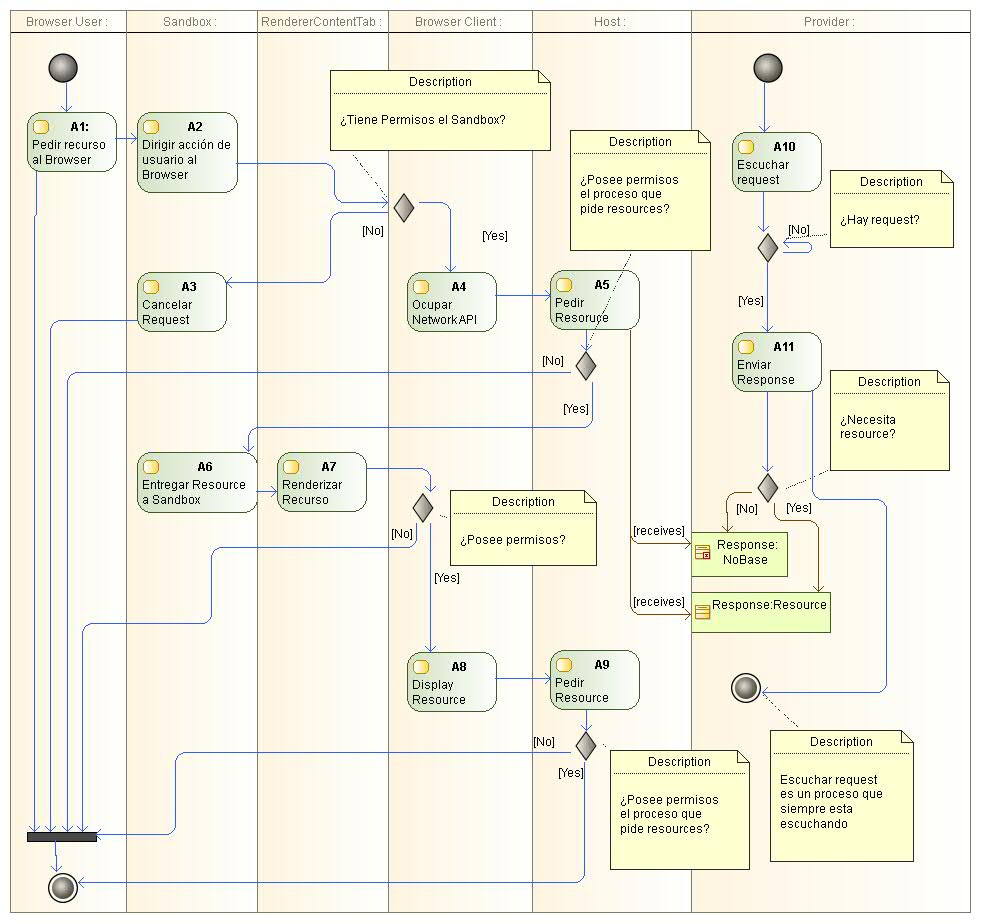
\includegraphics[scale=0.45]{figures/chap5/activityDiag.jpg}
    \caption{Diagrama de Actividad Compuesto para los casos de uso \textbf{Realizar Request} y \textbf{Recibir Request}.}
    \label{fig:ActDiagr}
\end{figure}

\begin{landscape}% Landscape page
\begin{table}[h!t]
\caption{Tabla con amenazas.}
\centering
\begin{tabular}{ |m{3.5em}|m{2.5em}|m{1.5em}|m{6em}|m{6em}|m{10em}|m{6em}|m{7em}|} 
\hline
Actor & Acción & ID & Sec. Attrib (CO/IN/AV/ACC) & Source (AIn/UIn/Out) & Descripción & Attacker & Asset\\
\hline
\multirow{5}{1em}{Browser User} & \multirow{5}{1em}{A1} & 1.1 & CO/IN & Out & Modificación de Tráfico/paquetes & Externo & Browser Client, Host\\ 
& & 1.2 & IN/CO & UIn/Out/In & Pedir recurso dentro del Host & Externo & Browser Client, Host\\
& & 1.3 & CO/IN/AV & UIn/Out & Contactar un Provider Malicioso & Externo & Browser Client, Host\\
& & 1.4 & CO & Out/UIn & Predecir comportamiento o análisis de tráfico & Externo, Process malicioso & Browser Client\\
& & 1.5 & CO/IN/ACC & Out & Conseguir contraseñas o información personal & Externo & Browser Client, Host\\
\hline
\multirow{4}{1em}{Host} & \multirow{5}{1em}{A5 y A9} & 5.1 & CO & Ain/UIn/Out & Divulgar información & Externo & Browser Client, Host\\ 
& & 5.2 & IN/CO & AIn/Out & Imitar a un Host honesto & Administrador Malicioso de Host & Browser Client, Provider\\
& & 5.3 & CO/IN/AV & Ain/Out/UIn & Contactar Provider Malicioso & Externo & Browser Client, Host\\
& & 5.4 & AV & Out & Impedir navegación & Externo & Browser Client\\
\hline
\multirow{2}{1em}{Provider} & \multirow{5}{1em}{A10} & 10.1 & IN/AV/ACC & Out & Aceptar request de cliente comprometido & Administrador Malicioso, Externo & Provider\\ 
& & 10.2 & CO & Ain/Out/UIn & Divulgar información & Externo & Provider\\

\hline
\end{tabular}
\label{tab:threats}
\end{table}
\end{landscape}

Hemos identificado algunas amenazas al analizar el curso de los eventos de los casos de uso: \textbf{Realizar Request} y \textbf{Recibir Request} (Figura \ref{fig:ActDiagr}). La tabla \ref{tab:threats} hace un sumario del análisis de cada acción en el diagrama de actividad, teniendo en cuenta los atributos de seguridad que podrían ser comprometidos, el origen de la amenaza y los recursos que pueden peligrar. Los atributos de seguridad principales son: Confidencialidad (CO), Integridad (IN), Disponibilidad (AV) y Responsabilidad (AC). El origen de la amenaza puede ser: actor autorizado (Ain), un actor no autorizado (UIn) o un externo (Out).
%Listar las amenazas que pueden ocurrir en el sistema no es suficiente para entender como los ataques ocurren. Es por esto que utilizaremos 2 patrones de mal uso, que permitirán describir como un ataque ocurre desde el punto de vista del atacante.

\section{Template de Patrones de Mal Uso}
\label{chap5:TemplateMP}
Esta sección describe cada parte del \textit{template} a usar para un Patron de Mal uso o Uso Indebido.

\subsection*{Nombre}
El nombre del patrón debe corresponder al nombre genérico dado al tipo específico de ataque en los repositorios estándares de ataques, como por el usado por el CERT \cite{cve}.

\subsection*{Intent o descripción básica}
Una descripción corta del propósito del patrón (qué problema resuelve para el atacante).

\subsection*{Contexto}
Describe el entorno genérico incluyendo las condiciones bajo a las cuales el ataque puede ocurrir. Esto puede incluir defensas mínimas presentes en el sistema, así como también vulnerabilidades típicas del sistema. El contexto puede ser especificado usando Diagramas de \textit{Deployment} de las partes relevantes del sistema así como también Diagaramas de Secuencia o de Colaboración que explayen el uso normal del sistema. Un diagrama de clases podría mostrar la estructura relevante del sistema. Se especifican además precondiciones para que el ataque ocurra.

\subsection*{Problema}
Desde la mirada del atacante, el problema es encontrar \textbf{cómo} atacar el sistema. Un problema adicional es cuando el sistema está protegido por mecanismos de defensa. Las fuerzas indican qué factores pueden ser requeridos en orden de ejecutar el ataque y en cómo realizarlo; por ejemplo, qué vulnerabilidades pueden ser explotadas. Además, qué factores podrían evitar que el ataque se pueda llevar acabo o lo retrasen.

\subsection*{Solución}
Esta sección describe la solución que resuelve el problema del atacante, ej: cómo el ataque puede alcanzar sus objetivos y los resultados esperados de éste. Diagramas en UML muestran los componentes del sistema involucrados. Diagramas de Secuencia o Colaboración muestran el intercambio de mensajes necesarios para cumplir con el ataque. Diagramas de actividad pueden añadir más detalle.

\subsection*{Componentes del sistema afectados (Dónde buscar evidencia)}
Esta sección adicional al \textit{template} original de un Patrón de Seguridad \cite{fernandez2013security} es nueva, dado que tiene relación con el mal uso realizado. La solución debe representar todos los componentes que están involucrados en el ataque, pero no debe ser una extensa lista, solo los más importantes para prevenirlo o lo escencial para una examinación forense. Esto puede ser representado por un diagrama de clases, que puede ser un subset o un superset del diagrama del contexto.

\subsection*{Usos comúnes}
Es prefeerido indicar los incidentes específicos en donde el ataque ha ocurrido. Pero en el caso de vulnerabilidades nuevas, donde el ataque aún puede que aún no se haya realizado, un contexto específico dónde el ataque pueda llevarse acabo es suficiente.

\subsection*{Consecuencias}
Discute los beneficios y desventajas del patrón de mal uso o uso indebido desde el punto de vista del atacante. ¿Es acaso el esfuerzo y costo gastado comparable a los resultados obtenidos? Esta es una evaluación que debe ser realizada por el atacante al decidir realizar el ataque; Diseñadores deben evaluar el riesgo de sus activos usando alpún enfoque de análisis de riesgos. La enumeración incluye buenos y malos aspectos, que deben ser emparejados a las fuerzas o \textit{forces}


\subsection*{Contramedidas y Evidencia Forense}
Esta sección describe las medidas de seguridad necesarias para detener, mitigar, o rastrear este tipo de ataque. Esto implica la enumeración de los Patrones de Seguridad o \textit{Security Patterns} que son efectivos contra este ataque. Desde un punto de vista Forense, se describe qué información puede ser obtenida en cada etapa rastreando el ataque y lo que puede ser deducido de los datos con el fin de identificar el ataque en específico. Finalmente, podría indicar qué información adicional debe ser recolectada en los componentes o unidades incolucrados para poder mejorar el análisis forense.

\subsection*{Patrones Similares}
Discute otros patrones de mal uso o uso indebido con diferentes objetivos pero realizados de manera similar, o con objetivos similares pero realizados de otra manera.

%PATRÓN

\section{Patrón de Mal Uso: Modificación de tráfico en el Web Browser}
En esta sección presentaremos un patrones de mal uso que describe la amenaza encontrada en el patrón Browser Infrastructure que hemos obtenido en este trabajo.
Una de las amenazas es que un atacante haya sido capaz de comprometer la respuesta obtenida desde el Provider contactado. El atacante podría tratar de reemplazar algunos parámetros de la respuesta del provider, entregando al Browser User un contenido distinto al original.

\subsection{Intent}
Un atacante podría cambiar contenido o dar uno diferente al esperado cuando el Web Browser (Browser User) recibe la response del Servidor o Provider. Realizando esta acción, el Navegador podría interpretar la información de una manera distinta a que si hubiera recibido el tráfico original.

\subsection{Contexto}
Un Navegador web obtiene resources desde un Provider para poder satisfacer un Browser User que lo necesita. Un Provider posee resources en forma de páginas web, servicios web u otro tipo. El Provider generalmente consiste en una Web App o Web server, que puede permitir entrada y salida de datos a otras aplicaciones, normalmente éstos están construidos usando HTML, Javascript y CCS. Sea que éste desea entregar servicios, como también otros deseen conectarse a él, todo tipo de comunicación estará encima del protocolo HTTP. Un Provider, dependiendo del tipo, puede llegar a recibir muchas peticiones de diversos Host para obtener recursos de éste. Dependiendo del tipo de peticiones, éstas pueden o no ser permitidas. Aquellas que son permitidas, el Provider generará una response a la \textit{request} del Host, la cuál terminará llegando de vuelta (o no) al Browser Client que generó el \textit{request}.

\subsection{Problema}
¿Cómo podría un atacante engañar al Browser User y Host, por medio de la modificación de tráfico entre las entidades participantes en la comunicación? Es posible que un atacante esté escondido entre medio de la comunicación que hay entre el Host y el Provider, lo que resulta en que el contenido modificado podría afectar dentro del RendererContentTab o el Browser Client. Esto en consecuencia podría traer diferentes resultados, desde el robo de información privada del Browser User que utiliza el Browser Client para personalizar la navegación como también los token de autenticación hacia los Providers que el Browser User ha utilizado previamente. Dependiendo del tipo de atacante, es posible que éste pueda incluso afectar al Host del Browser, dejando que el atacante pueda realizar actos maliciosos con los recursos del Host. 
El ataque puede sacar ventaja de las siguientes vulnerabilidades:
\begin{itemize}
	\item El \textbf{origen} u \textbf{origin} que define el Same Origin Policy que hace cumplir el Browser difiere en cada tipo de Web Browser \cite{W3C-SOP,Reis2009, Jackson2008, Crowley2010, Paola2006}.
	\item El \textbf{origin} no es suficiente como método de aislación entre resources (páginas web, scripts, css y otros) \cite{Silic2010, Barth2009, Yason, Liu2012}.
	\item Cualquiera puede crear una extensión o plugin, etc. para algún tipo de Browser y hacerlo pasar como algo inofensivo, pero el usuario no se daría cuenta que un ataque Man in the Browser podría estar ocurriendo \cite{Dougan2012,Utakrit2009,Liu2012,Barth2010}.  Éste programa, posiblemente malicioso, podría afectar el tráfico sin que queden rastros, pues tiene permisos del usuario al ser éste mismo quien autorizó su instalación.
	\item Es posible afectar al Browser Client, y en consecuencia al Host, sin tener que buscar vulnerabilidades en el Web Browser. Solamente utilizando métodos de ingeniería social, sobre el usuario del Host basta para lograr un ataque, pues es \textbf{el eslabón más débil}.
	\item La arquitectura para extender la funcionalidad del navegador, a través de extensiones, plugins y otros, depende demasiado del manufacturador. Y probablemente posee una gran superficie de ataque.
\end{itemize}

El ataque puede ser facilitado por:
\begin{itemize}
	\item Existen muchas herramientas para realizar ataques de ingeniería social, lo que permite hacer que el Browser User acepte realizar la instalación de extensiones o plugin maliciosos más fácilmente.
	\item Cualquier script basado en texto puede ser usado para explotar el intérprete del navegador web. Muchas veces también es posible utilizar los mismos elementos del lenguaje de scripting para poder pasar ciertas barreras de seguridad entregadas por el SOP, pues el lenguaje está basado en prototipos. 
	\item Los manufacturadores de Navegadores no poseen aún mecanismos de defensa que permitan identificar efectivamente cuando un recurso puede ser malicioso.
	\item Los métodos de cifrado no pueden hacer nada contra un ataque que puede modificar el tráfico antes de enviar o después de recibir el mensaje.
	\item No existen mecanismos de defensa estandarizados, pues cada manufacturador realiza lo necesario para la marca a la que se acopla. Si el Host posee muchos browser, la superficie de ataque es bastante mayor.
\end{itemize}
\subsection{Solución}
La solución estructural usada es la misma creada por el patrón Browser Infrastructure que se revisó en el capítulo 4. La clase Attacker es cualquier entidad que podría llevar a cabo una acción arriesgada contra la integridad del Browser, usuario, Host y Provider (Figura \ref{fig:BIMisuse}). El atacante es capaz tanto de interceptar las response que el Provider envía al Browser Client usando al Host como receptor, o haciendo que el Browser realice modificaciones en el input que va hacia el Provider, utilizando scripts u otro resources.
\begin{figure}[h!t]
	        \centering
	        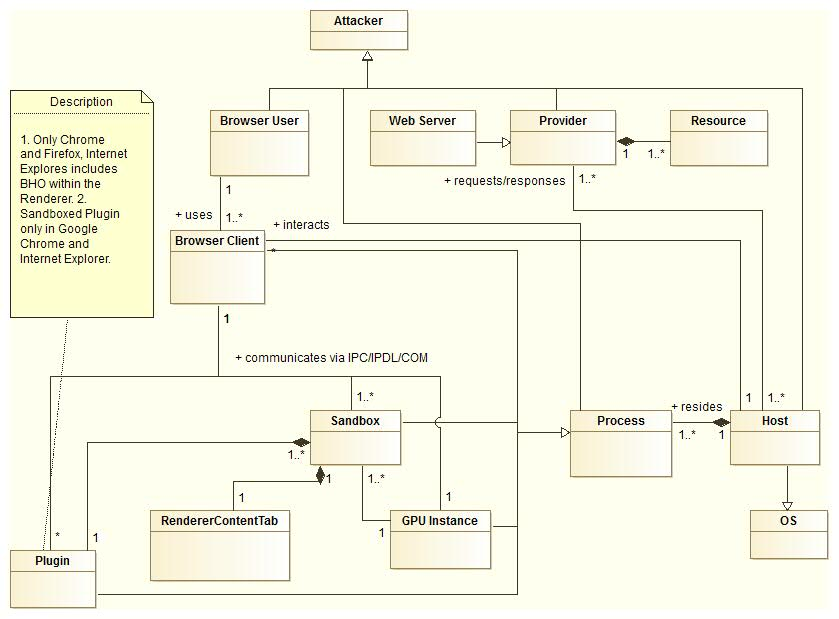
\includegraphics[scale=0.45]{figures/chap5/patronMisuse.jpg}
	        \caption{Diagrama de Clases para el patrón de Misuse.}
	        \label{fig:BIMisuse}
    \end{figure}

\subsection{Dinámica}
En la figura \ref{fig:SeqMisuse} se muestra la serie de pasos necesarios, para realizar uno de los tantos mal usos que se pueden realizar durante el caso de uso Realizar \textit{request}. El atacante queda entre el Browser Client y el Host, interceptando la realización del \textit{request} original y modificando el tráfico a su gusto; usualmente un ataque basado en este mal uso se le llama Man-in-the-Browser (MITB) \cite{Liu2012, Barth2010, Utakrit2009, Dougan2012}. Esto podría perfectamente suceder cuando el Browser User ha permitido la instalación de plugins, extensiones o programas externos en el Host y Browser Client [ref]
\begin{figure}[h!t]
	        \centering
	        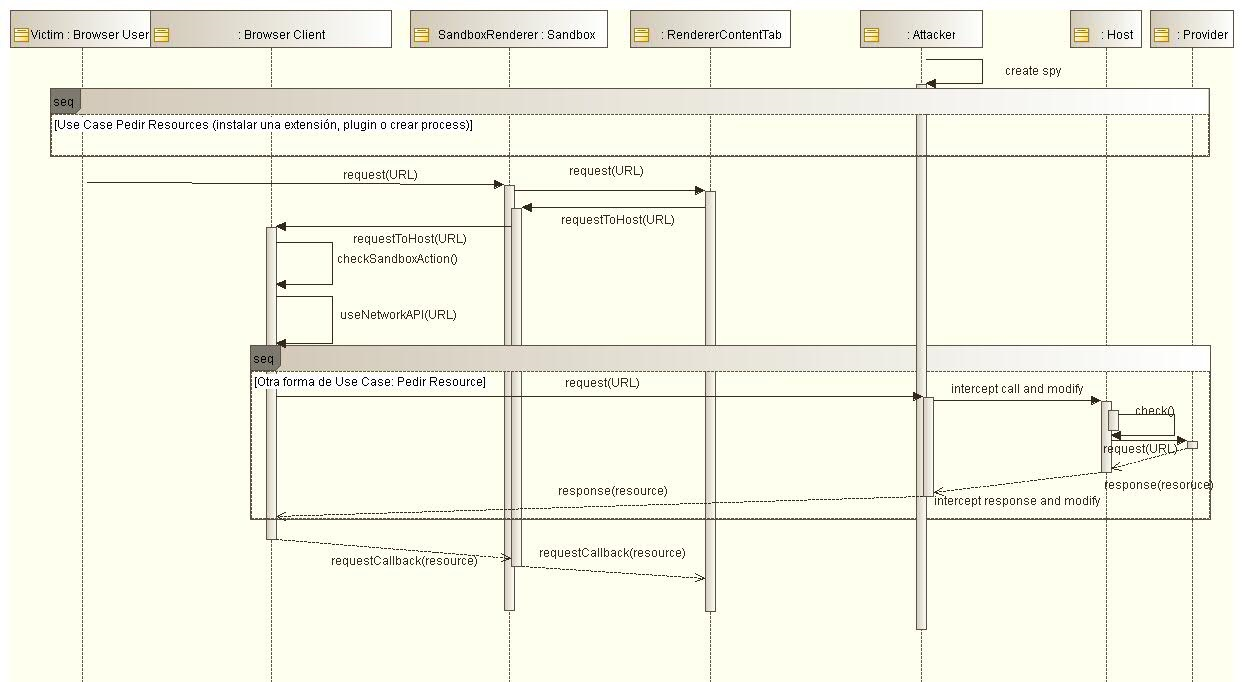
\includegraphics[scale=0.45]{figures/chap5/patronMisuseSeq.jpg}
	        \caption{Diagrama de Secuencia para el Mal uso: Modificación de tráfico en el Web Browser.}
	        \label{fig:SeqMisuse}
    \end{figure}
	
	\subsubsection{Sumario} El atacante intercepta el tráfico entre Host y Browser Client.
	\subsubsection{Actor} Atacante
	\subsubsection{Precondiciones} Para que el ataque pueda pasar desapercibido, es necesario que el Browser User o el usuario detrás del browser haya caído primero en un ataque de ingeniería social o el atacante haya podido instalar directamente un proceso o componente malicioso en el Host directamente.
	\subsubsection{Descripción}
			\begin{enumerate}
				\item Un atacante utiliza alguna técnica de ingeniería social o vulnerabilidad en el sistema, para crear una entidad que se encargará de estar entre medio del Browser Client y el Provider. Para esto realiza el caso de uso \textbf{Pedir Resources} para que el proceso, plugin o extensión se aloje en el Host.
				\item Un Browser Consumer desea hacer un \textit{request} a cierta URL, por lo que los primeros pasos de \textbf{Realizar Request} son similares.
				\item En el momento en que el Browser Client va a realizar la llamada al sistema para enviar el mensaje del Host al Provider, el Browser Client llamará al plugin, extensión o process malicioso, pues el Browser Client ha sido intervenido para que realice esa acción de este modo.
				\item El atacante entonces recibirá todo el tráfico del Browser Client, el cuál podría modificar a su antojo.
				\item Finalmente la víctima está totalmente comprometida.
			\end{enumerate}
	\subsubsection{Post condiciones} La víctima quedará completamente comprometida y probablemente no sea posible detectar la alteración del mensaje, pues también es posible que se modifiquen los log del Host.
	\subsubsection{Usos Conocidos} El Web Browser es un software que posee diversas implementaciones, por lo tanto la cantidad de vectores de ataque es significativa. Algunos de éstos son:
			\begin{itemize}
				\item  Una extensión basada en la arquitectura de Chrome o la API WebExtension Firefox, podría interceptar los datos antes que llegue al Browser Client \cite{Paola2006} o dado a una vulnerabilidad del mismo elemento un atacante se está aprovechando de su funcionalidad para realizar ataques \cite{Liu2012, Barth2010}. Dado que el Plugin, la extensión o el process son elementos que el Host confía, es posible que el ataque sea indetectable y los métodos de cifrado no sirven como medida de mitigación.
				\item Éste tipo de ataque puede ser usado como base para otros ataques más avanzados. Un ejemplo es cuando el Browser posee vulnerabilidades \textit{cross-origin javascript capability leaks}, donde los diferentes modelos de seguridad usados por Javascript y el DOM pueden interferir entre sí, causando que una petición \textit{cross-origin} se pueda realizar aún cuando SOP debería ser capaz de detener tal ataque \cite{Barth2009}.
			\end{itemize}


\subsection{Consecuencias}
	El mal uso tiene las siguientes consecuencias para el Attacker:
	\begin{itemize}
		\item Objetivos: pueden ser diversos, destacándose el vandalismo, personificar a otra persona u obtener una ganancia monetaria. Mientras el atacante se pueda interponer entre el Host y el tráfico que se envía al Provider, la confidencialidad e integridad de los datos está completamente perdida. La privacidad del usuario ya no se puede asegurar tampoco.
		\item Silencioso: Dado que el atacante ha logrado interponerse entre las llamadas de sistema que se realizan al Host para enviar los datos al Provider, el Host no reconocerá ni logueará ninguna anomalía. Las llamadas hechas al Host son totalmente legales y nada fuera de lo normal para éste.
		\item El atacante podría realizar acciones que afecten la integridad del Host.
	\end{itemize}
	Posibles fuentes de fallo:
	\begin{itemize}
		\item Si el Browser User es capaz de evitar o ignorar el ataque de Ingeniería Social realizado al comienzo, no existiría este mal uso. Esto debe considerar que el usuario también no se encuentre con páginas o contenido malicioso, que podrían afectar otro componente de Browser, pero que causarían en el mismo efecto del Mal Uso señalado.
	\end{itemize}

\subsection{Contramedidas} 
	Para prevenir este tipo de mal uso se recomienda tomar las siguientes medidas preventivas:
	\begin{itemize}
		\item Servicios de Reputación como Smart Screen de Internet Explorer y Download Application de Google Chrome, ayudan a identificar páginas y contenido/resources que podrían contener malware que se instale como plugins, entensiones o process en el Host del Browser User.
		\item Entregando educación sobre los peligros de navegar por Internet y aclarar al usuario que él es la última línea de defensa contra éste tipo de ataques.
		\item White y Black list instaladas en los browser son una medida preventiva para evitar la navegación en páginas o recursos maliciosos ya conocidos.
		\item Navegadores como Google Chrome e Internet Explorer ofrecen el Sandboxing. Éste mecanismo de defensa limita las acciones del atacante, que pudieran afectar la integridad del sistema.
	\end{itemize}

\subsection{Evidencia Forense}
	¿Dónde es posible encontrar evidencia?
	Dependiendo de lo deseado por el atacante, las acciones que cometerá pueden diferir. Sin embargo el log interno del browser debería de poder servir para auditar el sistema, esto gracias a que mientras no se haya encontrado una vulnerabilidad en el Sandbox del Browser, el atacante no puede borrar completamente sus huellas.

\subsection{Patrones relacionados}
	\begin{itemize}
		\item En el patrón Browser Infrastructure, el Browser Client actúa como el Reference Monitor explicado en \cite{fernandez2001pattern}.
	\end{itemize}
